
\documentclass[a4paper,11pt]{article}
\usepackage[a4paper, margin=8em]{geometry}

% usa i pacchetti per la scrittura in italiano
\usepackage[french,italian]{babel}
\usepackage[T1]{fontenc}
\usepackage[utf8]{inputenc}
\frenchspacing 

% usa i pacchetti per la formattazione matematica
\usepackage{amsmath, amssymb, amsthm, amsfonts}

% usa altri pacchetti
\usepackage{gensymb}
\usepackage{hyperref}
\usepackage{standalone}

\usepackage{colortbl}

\usepackage{xstring}
\usepackage{karnaugh-map}

% imposta il titolo
\title{Electronics for Embedded Systems notes}
\author{Luca Seggiani}
\date{2026}

% spaziatura liste
\usepackage{enumitem}
\setlist[itemize]{noitemsep, topsep=4pt, partopsep=0pt, parsep=2pt, leftmargin=*}
\setlist[enumerate]{noitemsep, topsep=4pt, partopsep=0pt, parsep=2pt, leftmargin=*}

% imposta lo stile
% usa helvetica
\usepackage[scaled]{helvet}
% usa palatino
\usepackage{palatino}
% usa un font monospazio guardabile
\usepackage{lmodern}

\renewcommand{\rmdefault}{ppl}
\renewcommand{\sfdefault}{phv}
\renewcommand{\ttdefault}{lmtt}

% circuiti
\usepackage{circuitikz}
\usetikzlibrary{babel}

% testo cerchiato
\newcommand*\circled[1]{\tikz[baseline=(char.base)]{
            \node[shape=circle,draw,inner sep=2pt] (char) {#1};}}

% disponi il titolo
\makeatletter
\renewcommand{\maketitle} {
	\begin{center} 
		\begin{minipage}[t]{.8\textwidth}
			\textsf{\huge\bfseries \@title} 
		\end{minipage}%
		\begin{minipage}[t]{.2\textwidth}
			\raggedleft \vspace{-1.65em}
			\textsf{\small \@author} \vfill
			\textsf{\small \@date}
		\end{minipage}
		\par
	\end{center}

	\thispagestyle{empty}
	\pagestyle{fancy}
}
\makeatother

% disponi teoremi
\usepackage{tcolorbox}
\newtcolorbox[auto counter, number within=section]{theorem}[2][]{%
	colback=blue!10, 
	colframe=blue!40!black, 
	sharp corners=northwest,
	fonttitle=\sffamily\bfseries, 
	title=Theorem~\thetcbcounter: #2, 
	#1
}

% disponi definizioni
\newtcolorbox[auto counter, number within=section]{definition}[2][]{%
	colback=red!10,
	colframe=red!40!black,
	sharp corners=northwest,
	fonttitle=\sffamily\bfseries,
	title=Definition~\thetcbcounter: #2,
	#1
}

% disponi codice
\usepackage{listings}
\usepackage[table]{xcolor}

\definecolor{codegreen}{rgb}{0,0.6,0}
\definecolor{codegray}{rgb}{0.5,0.5,0.5}
\definecolor{codepurple}{rgb}{0.58,0,0.82}
\definecolor{backcolour}{rgb}{0.95,0.95,0.92}

\lstdefinestyle{codestyle}{
		backgroundcolor=\color{black!5}, 
		commentstyle=\color{codegreen},
		keywordstyle=\bfseries\color{magenta},
		numberstyle=\sffamily\tiny\color{black!60},
		stringstyle=\color{green!50!black},
		basicstyle=\ttfamily\footnotesize,
		breakatwhitespace=false,         
		breaklines=true,                 
		captionpos=b,                    
		keepspaces=true,                 
		numbers=left,                    
		numbersep=5pt,                  
		showspaces=false,                
		showstringspaces=false,
		showtabs=false,                  
		tabsize=2
}

\lstdefinestyle{shellstyle}{
		backgroundcolor=\color{black!5}, 
		basicstyle=\ttfamily\footnotesize\color{black}, 
		commentstyle=\color{black}, 
		keywordstyle=\color{black},
		numberstyle=\color{black!5},
		stringstyle=\color{black}, 
		showspaces=false,
		showstringspaces=false, 
		showtabs=false, 
		tabsize=2, 
		numbers=none, 
		breaklines=true
}

\lstdefinelanguage{x86}{ 
  keywords={AAA, AAD, AAM, AAS, ADC, ADCB, ADCW, ADCL, ADD, ADDB, ADDW, ADDL, AND, ANDB, ANDW, ANDL,
        ARPL, BOUND, BSF, BSFL, BSFW, BSR, BSRL, BSRW, BSWAP, BT, BTC, BTCB, BTCW, BTCL, BTR, 
        BTRB, BTRW, BTRL, BTS, BTSB, BTSW, BTSL, CALL, CBW, CDQ, CLC, CLD, CLI, CLTS, CMC, CMP,
        CMPB, CMPW, CMPL, CMPS, CMPSB, CMPSD, CMPSW, CMPXCHG, CMPXCHGB, CMPXCHGW, CMPXCHGL,
        CMPXCHG8B, CPUID, CWDE, DAA, DAS, DEC, DECB, DECW, DECL, DIV, DIVB, DIVW, DIVL, ENTER,
        HLT, IDIV, IDIVB, IDIVW, IDIVL, IMUL, IMULB, IMULW, IMULL, IN, INB, INW, INL, INC, INCB,
        INCW, INCL, INS, INSB, INSD, INSW, INT, INT3, INTO, INVD, INVLPG, IRET, IRETD, JA, JAE,
        JB, JBE, JC, JCXZ, JE, JECXZ, JG, JGE, JL, JLE, JMP, JNA, JNAE, JNB, JNBE, JNC, JNE, JNG,
        JNGE, JNL, JNLE, JNO, JNP, JNS, JNZ, JO, JP, JPE, JPO, JS, JZ, LAHF, LAR, LCALL, LDS,
        LEA, LEAVE, LES, LFS, LGDT, LGS, LIDT, LMSW, LOCK, LODSB, LODSD, LODSW, LOOP, LOOPE,
        LOOPNE, LSL, LSS, LTR, MOV, MOVB, MOVW, MOVL, MOVSB, MOVSD, MOVSW, MOVSX, MOVSXB,
        MOVSXW, MOVSXL, MOVZX, MOVZXB, MOVZXW, MOVZXL, MUL, MULB, MULW, MULL, NEG, NEGB, NEGW,
        NEGL, NOP, NOT, NOTB, NOTW, NOTL, OR, ORB, ORW, ORL, OUT, OUTB, OUTW, OUTL, OUTSB, OUTSD,
        OUTSW, POP, POPL, POPW, POPB, POPA, POPAD, POPF, POPFD, PUSH, PUSHL, PUSHW, PUSHB, PUSHA, 
        RCLL, RCR, RCRB, RCRW, RCRL, RDMSR, RDPMC, RDTSC, REP, REPE, REPNE, RET, ROL, ROLB, ROLW,
        ROLL, ROR, RORB, RORW, RORL, SAHF, SAL, SALB, SALW, SALL, SAR, SARB, SARW, SARL, SBB,
        SBBB, SBBW, SBBL, SCASB, SCASD, SCASW, SETA, SETAE, SETB, SETBE, SETC, SETE, SETG, SETGE,
        SETL, SETLE, SETNA, SETNAE, SETNB, SETNBE, SETNC, SETNE, SETNG, SETNGE, SETNL, SETNLE,
        SETNO, SETNP, SETNS, SETNZ, SETO, SETP, SETPE, SETPO, SETS, SETZ, SGDT, SHL, SHLB, SHLW,
        SHLL, SHLD, SHR, SHRB, SHRW, SHRL, SHRD, SIDT, SLDT, SMSW, STC, STD, STI, STOSB, STOSD,
        STOSW, STR, SUB, SUBB, SUBW, SUBL, TEST, TESTB, TESTW, TESTL, VERR, VERW, WAIT, WBINVD,
        XADD, XADDB, XADDW, XADDL, XCHG, XCHGB, XCHGW, XCHGL, XLAT, XLATB, XOR, XORB, XORW, XORL},
  keywordstyle=\color{blue}\bfseries,
  ndkeywordstyle=\color{darkgray}\bfseries,
  identifierstyle=\color{black},
  sensitive=false,
  comment=[l]{\#},
  morecomment=[s]{/*}{*/},
  commentstyle=\color{purple}\ttfamily,
  stringstyle=\color{red}\ttfamily,
  morestring=[b]',
  morestring=[b]"
}

\lstdefinelanguage{riscv}{
  keywords={
    LUI, AUIPC,
    JAL, JALR,
    BEQ, BNE, BLT, BGE, BLTU, BGEU,
    LB, LH, LW, LBU, LHU, LD,
    SB, SH, SW, SD,
    ADDI, SLTI, SLTIU, XORI, ORI, ANDI,
    SLLI, SRLI, SRAI,
    ADD, SUB, SLL, SLT, SLTU, XOR, SRL, SRA, OR, AND,
    ADDIW, SLLIW, SRLIW, SRAIW,
    ADDW, SUBW, SLLW, SRLW, SRAW,
    MUL, MULH, MULHSU, MULHU, DIV, DIVU, REM, REMU,
    MULW, DIVW, DIVUW, REMW, REMUW,
    LR.W, SC.W, AMOSWAP.W, AMOADD.W, AMOXOR.W,
    AMOAND.W, AMOOR.W, AMOMIN.W, AMOMAX.W,
    AMOMINU.W, AMOMAXU.W,
    LR.D, SC.D, AMOSWAP.D, AMOADD.D, AMOXOR.D,
    AMOAND.D, AMOOR.D, AMOMIN.D, AMOMAX.D,
    AMOMINU.D, AMOMAXU.D,
    FLW, FSW,
    FMADD.S, FMSUB.S, FNMSUB.S, FNMADD.S,
    FADD.S, FSUB.S, FMUL.S, FDIV.S, FSQRT.S,
    FSGNJ.S, FSGNJN.S, FSGNJX.S,
    FMIN.S, FMAX.S,
    FCVT.W.S, FCVT.WU.S, FCVT.S.W, FCVT.S.WU,
    FMV.X.W, FMV.W.X,
    FEQ.S, FLT.S, FLE.S,
    FLD, FSD,
    FMADD.D, FMSUB.D, FNMSUB.D, FNMADD.D,
    FADD.D, FSUB.D, FMUL.D, FDIV.D, FSQRT.D,
    FSGNJ.D, FSGNJN.D, FSGNJX.D,
    FMIN.D, FMAX.D,
    FCVT.W.D, FCVT.WU.D, FCVT.D.W, FCVT.D.WU,
    FCVT.S.D, FCVT.D.S,
    FMV.X.D, FMV.D.X,
    FEQ.D, FLT.D, FLE.D,
    CSRRW, CSRRS, CSRRC,
    CSRRWI, CSRRSI, CSRRCI,
    FENCE.I,
    FENCE,
    ECALL, EBREAK,
    MRET, SRET, URET,
    WFI,
    SFENCE.VMA,
    NOP, LI, LA, MV,
    NOT, NEG, NEGW,
    SEQZ, SNEZ, SLTZ, SGTZ,
    BEQZ, BNEZ, BLEZ, BGEZ, BLTZ, BGTZ,
    BGT, BLE, BGTU, BLEU,
    J, JR, RET,
    CALL, TAIL,
    RDINSTRET, RDCYCLE, RDTIME,
    CSRR, CSRW, CSRS, CSRC,
    CSRWI, CSRSI, CSRCI
  },
  keywordstyle=\color{blue}\bfseries,
  ndkeywordstyle=\color{darkgray}\bfseries,
  identifierstyle=\color{black},
  sensitive=false,
  comment=[l]{\#},
  morecomment=[s]{/*}{*/},
  commentstyle=\color{purple}\ttfamily,
  stringstyle=\color{red}\ttfamily,
  morestring=[b]',
  morestring=[b]"
}

\lstdefinelanguage{arm}{
  keywords={
    ADC, ADD, AND, BIC, CMN, CMP, EOR, MOV, MVN,
    RSB, RSC, SBC, SUB, TST, TEQ,
    MLA, MLS, MUL, SMLAL, SMULL, UMLAL, UMULL,
    QADD, QSUB, QDADD, QDSUB,
    QADD16, QADD8, QASX, QSAX,
    QSUB16, QSUB8, QSAX, QSUBADDX,
    ASR, LSL, LSR, ROR, RRX,
    B, BL, BX, BLX,
    BXJ,
    BEQ, BNE, BCS, BHS, BCC, BLO,
    BMI, BPL, BVS, BVC,
    BHI, BLS, BGE, BLT, BGT, BLE,
    BAL,
    LDR, LDRB, LDRH, LDRSB, LDRSH,
    LDRD, LDM, LDMIA, LDMIB, LDMDA, LDMDB,
    LDRT, LDRBT, LDRHT, LDRSBT, LDRSHT,
    STR, STRB, STRH, STRD,
    STM, STMIA, STMIB, STMDA, STMDB,
    STRT, STRBT, STRHT,
    PUSH, POP,
    SWP, SWPB,
    REV, REV16, REVSH,
    BFC, BFI, BFXIL, SBFX, UBFX,
    CLZ,
    LDREX, LDREXB, LDREXH, LDREXD,
    STREX, STREXB, STREXH, STREXD,
    DMB, DSB, ISB,
    MCR, MCRR, MRC, MRRC,
    MRS, MSR,
    CPS, SETEND, SVC, BKPT,
    CLREX, WFE, WFI, SEV,
    YIELD, NOP,
    VLDR, VSTR,
    VMOV, VABS, VNEG,
    VADD, VSUB, VMUL, VDIV,
    VMLA, VMLS, VNMLA, VNMLS, VNMUL,
    VMAX, VMIN,
    VSQRT,
    VCMP, VCMPE,
    VCVT,
    VCLZ, VCLS,
    VAND, VORR, VEOR, VBIC, VMVN,
    VLD1, VLD2, VLD3, VLD4,
    VST1, VST2, VST3, VST4,
    ADR, ADCS, ADDS, SUBS, MOVS, ANDS, ORRS, EORS
  },
  keywordstyle=\color{blue}\bfseries,
  ndkeywordstyle=\color{darkgray}\bfseries,
  identifierstyle=\color{black},
  sensitive=false,
  comment=[l]{@},
  morecomment=[l]{;},
  morecomment=[s]{/*}{*/},
  commentstyle=\color{purple}\ttfamily,
  stringstyle=\color{red}\ttfamily,
  morestring=[b]',
  morestring=[b]"
}

\lstset{style=codestyle, language=C}

% disponi sezioni
\usepackage{titlesec}

\titleformat{\section}
	{\sffamily\Large\bfseries} 
	{\thesection}{1em}{} 
\titleformat{\subsection}
	{\sffamily\large\bfseries}   
	{\thesubsection}{1em}{} 
\titleformat{\subsubsection}
	{\sffamily\normalsize\bfseries} 
	{\thesubsubsection}{1em}{}

% tikz
\usepackage{tikz}

% float
\usepackage{float}

% grafici
\usepackage{pgfplots}
\pgfplotsset{width=10cm,compat=1.9}

% disponi alberi
\usepackage{forest}

\forestset{
	rectstyle/.style={
		for tree={rectangle,draw,font=\large\sffamily}
	},
	roundstyle/.style={
		for tree={circle,draw,font=\large}
	}
}

% disponi algoritmi
\usepackage{algorithm}
\usepackage{algorithmic}
\makeatletter
\renewcommand{\ALG@name}{Algorithm}
\makeatother

% disponi numeri di pagina
\usepackage{fancyhdr}
\fancyhf{} 
\fancyfoot[L]{\sffamily{\thepage}}

\makeatletter
\fancyhead[L]{\raisebox{1ex}[0pt][0pt]{\sffamily{\@title \ \@date}}} 
\fancyhead[R]{\raisebox{1ex}[0pt][0pt]{\sffamily{\@author}}}
\makeatother

\begin{document}
% sezione (data)
\section{Lesson 29-10-26}

% stili pagina
\thispagestyle{empty}
\pagestyle{fancy}

% testo
\subsection{Synchronous protocols}

In the last lesson we saw serial protocols, more specifically UART.
UART uses separate clocks at RX and TX, with synchronization on the START bit.

We know want to see protocols, either character or bit oriented, where clock recovery uses transitions of the data signal, in each bit (synchronous carrier), so periodically.

First some constraints:
The \textit{channel bandwidth} requirement is that it contains at  least the highest fundamental frequency in the transmitted signal.
The lower, the better, given a certain Bit Rate $f_\text{ck}$, as it makes for a cheaper channel.
This means we need to find the worst case depending on the bits transmitted.

For the number of \textit{voltage levels} used in the channel, we stick with standard logic which uses 2: $0 \, \mathrm{V}$ and $V_{dd}$.

\subsubsection{NRZ encoding}

A first approach is \textbf{NRZ} (\textit{Non Return to Zero Encoding}).
Several types:
\begin{itemize}
\item \textbf{NRZ-L} (\textit{Level}):
\begin{itemize}
\item Logic 1: high state
\item Logic 0: low state
\end{itemize}
\item \textbf{NRZ-M} (\textit{Mark}, also known as \textbf{NRZ-I}, \textit{Inverted}):
\begin{itemize}
\item Logic 1: represented by a transition
\item Logic 0: no change
\end{itemize}
\item \textbf{NRZ-S} (\textit{Space}, also known as \textbf{NRZ-I}, \textit{Inverted}):
\begin{itemize}
\item Logic 1: no change
\item Logic 0: represented by a transition
\end{itemize}
\end{itemize}

Note that in none of these transitions are \textit{guaranteed}! We might not have them, which prevents us from synchronizing on that clock cycle.

Also, since at most we change value once per clock, the maximum frequency for NRZ is:
$$
 f_\text{max} = \frac{f_\text{ck}}{2}
$$

\begin{center}
	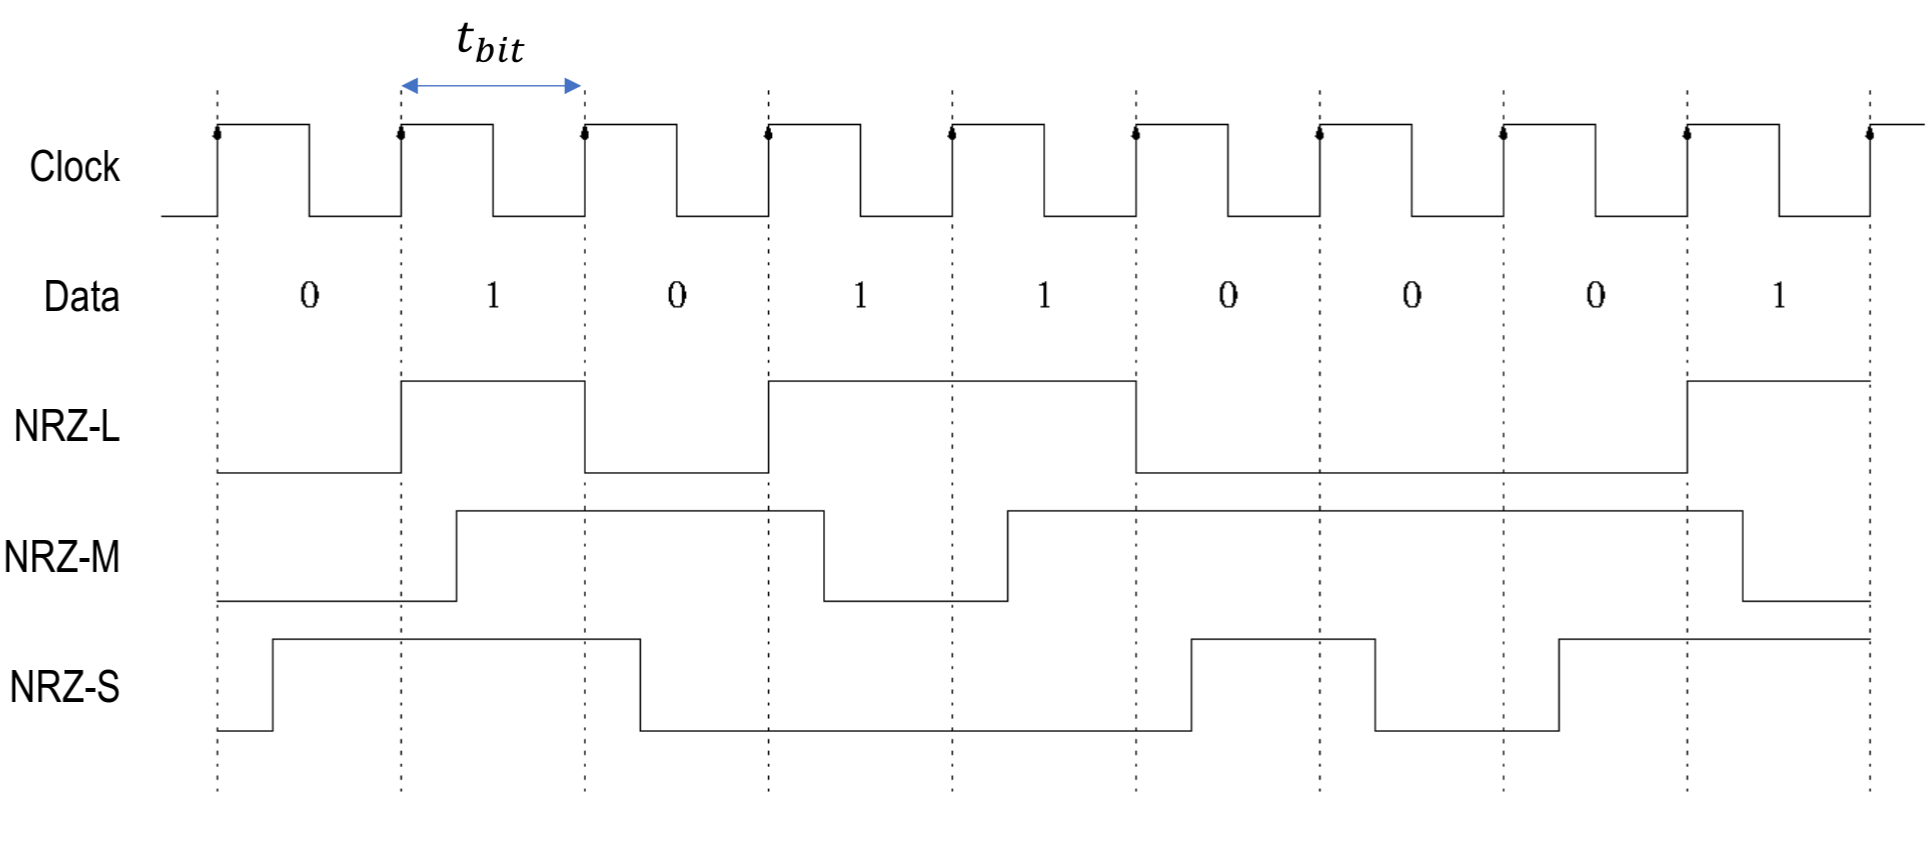
\includegraphics[scale=0.22]{../figures/nrz.png}
\end{center}

\subsubsection{RZ encoding}

The alternative is \textbf{RZ} (\textit{Return to Zero Encoding}). Several types of this too:
\begin{itemize}
\item Unipolar \textbf{RZ-M}
\begin{itemize}
\item Logic 1: high pulse
\item Logic 0: low state
\end{itemize}
\item Bipolar \textbf{RZ}
\begin{itemize}
\item Logic 1: positive pulse
\item Logic 0: negative pulse
\end{itemize}
\end{itemize}

Transitions are not guaranteed in unipolar, but they are in bipolar (good!), tough it needs a ternary code with better SNR.

For the bandwidth, we can change the value two times per clock, so the maximum frequency for both RZ types is:
$$
f_\text{max} = f_\text{ck}
$$

\begin{center}
	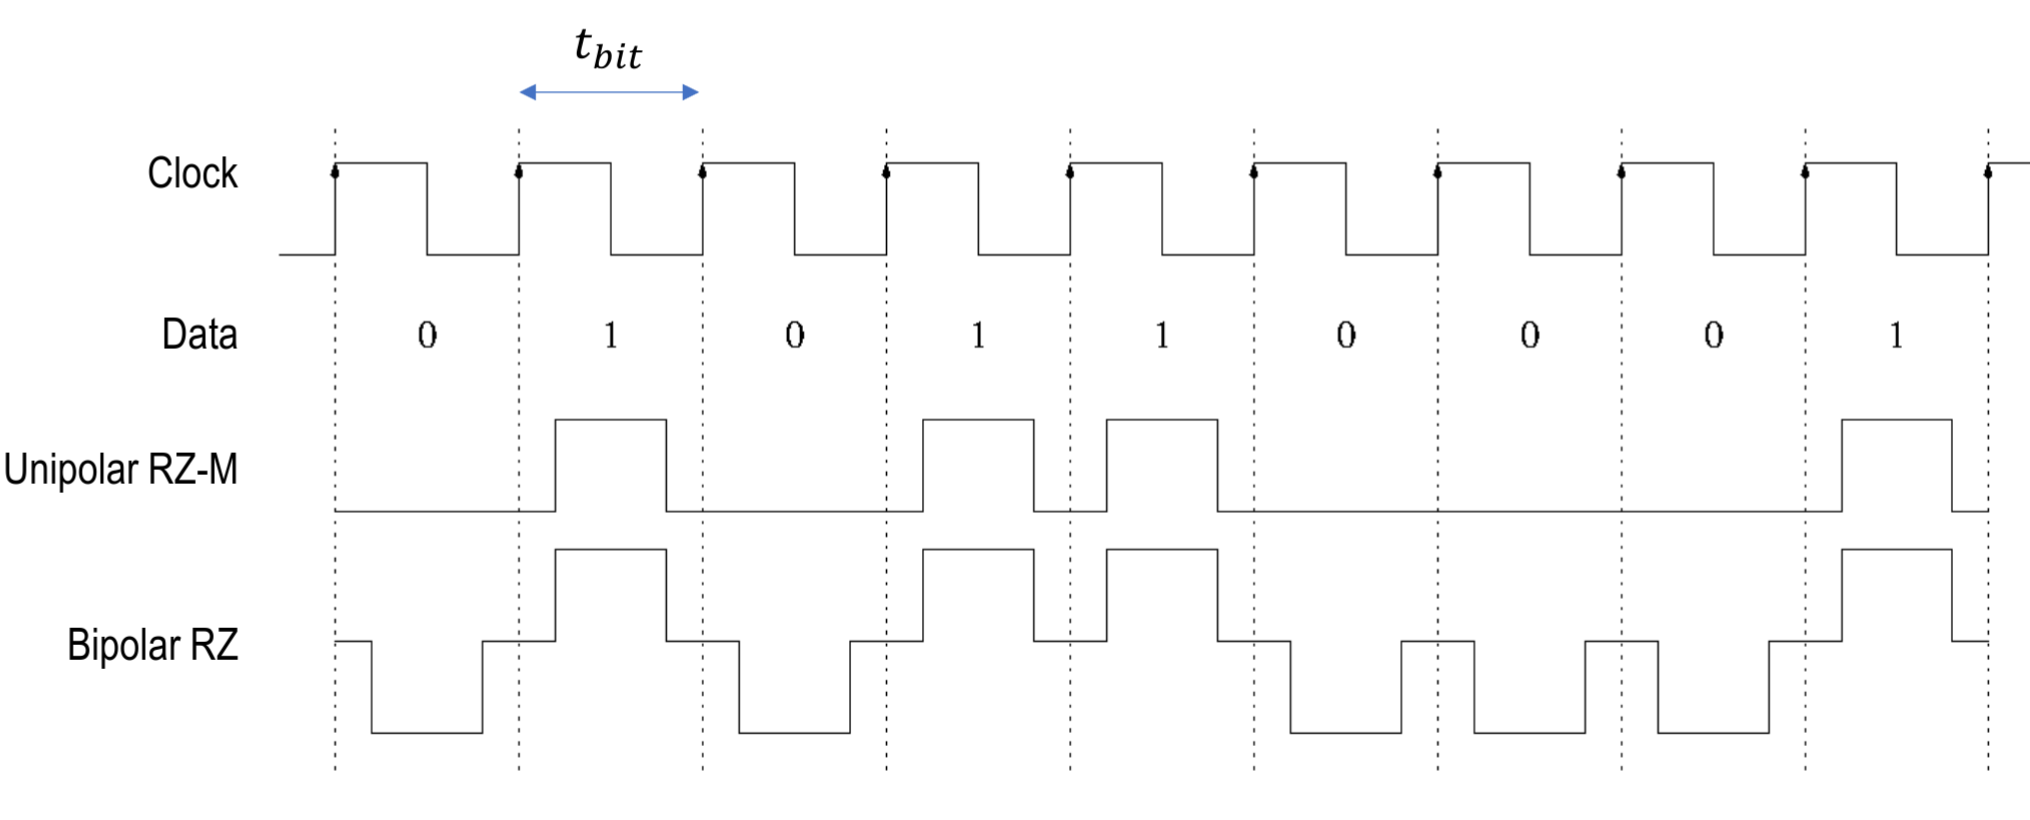
\includegraphics[scale=0.22]{../figures/rz.png}
\end{center}

\par\smallskip

An alternative that exists is \textbf{AMI} RZ (\textit{Alternative Mark Inverted Return to Zero}).
This involves marking:
\begin{itemize}
	\item Logic 1: alternate level pulse
	\item Logic 0: no pulse
\end{itemize}

Where, by alternate level pulse we mean a pulse opposite of the previous one.
We consider this because we find that the maximum frequency is in fact reduced:
$$
f_\text{max} = \frac{f_\text{ck}}{2}
$$

This is because the worst case scenario, where we transmit a high value at each cycle, gets us basically a sinusoidal wave at frequency $\frac{f_\text{ck}}{2}$.
Also, the DC component is absent on average, which is an advantage in long connections.

The tradeoff is that this clearly doesn't guarantee transitions. 

\begin{center}
	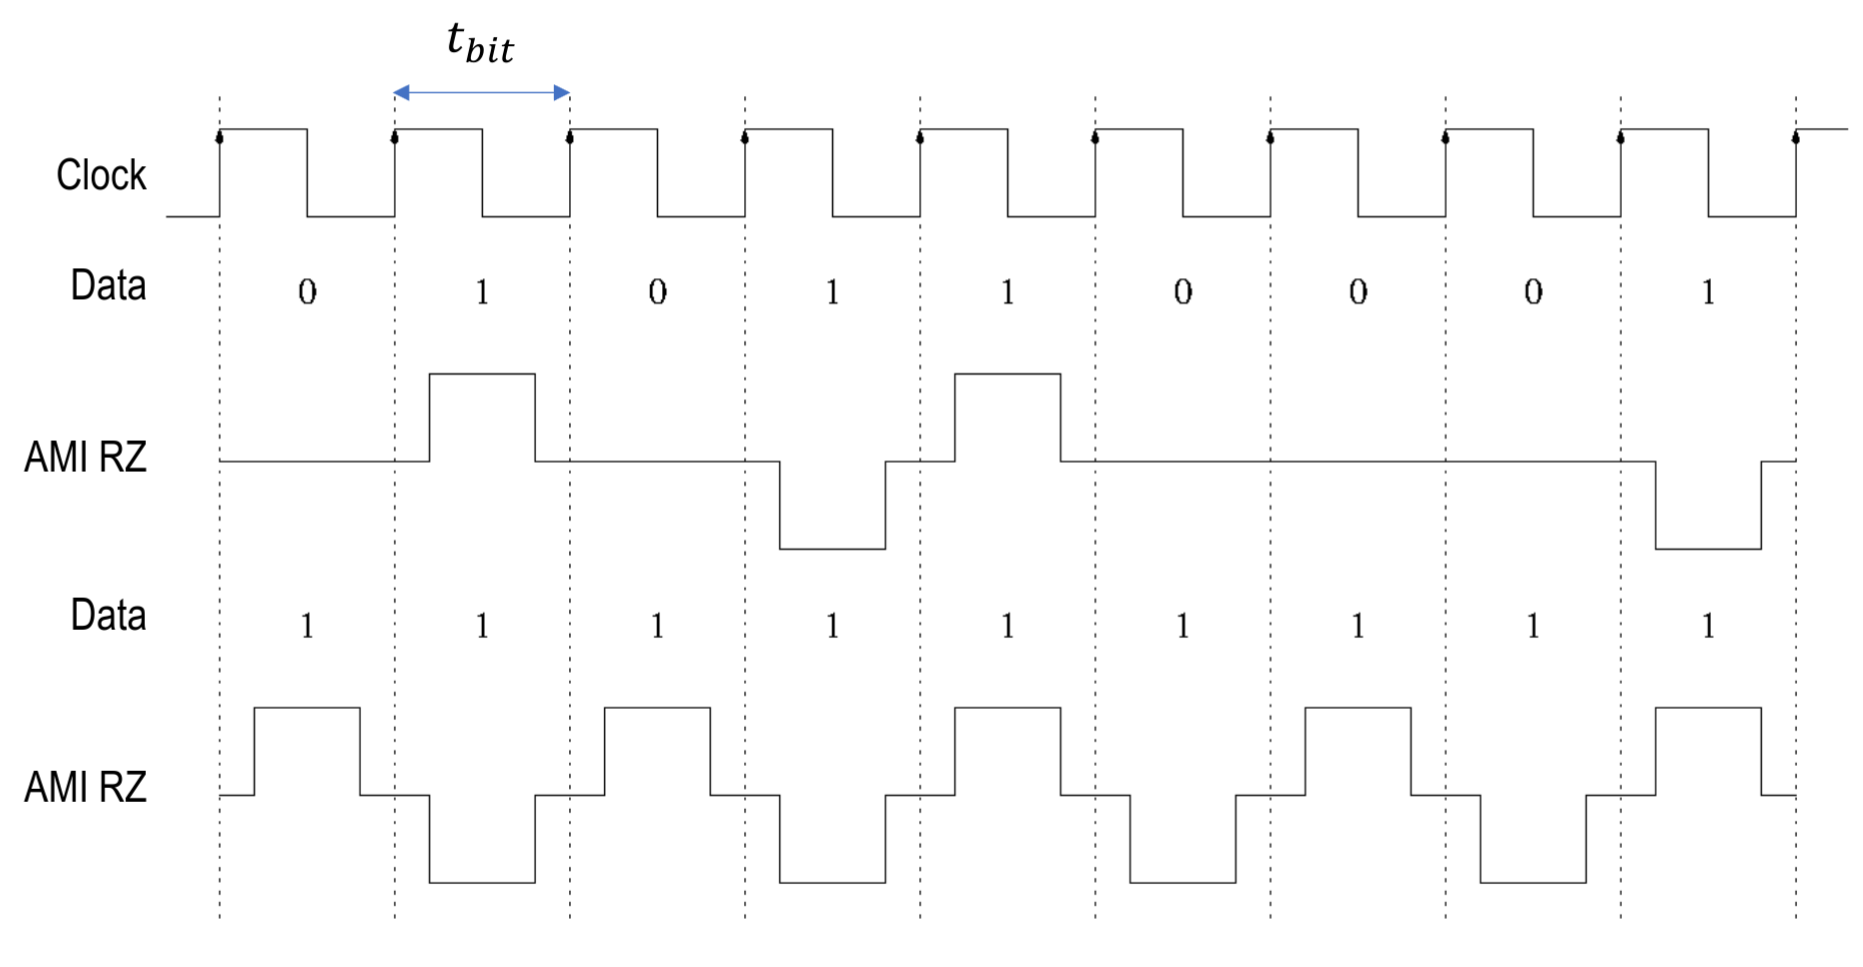
\includegraphics[scale=0.22]{../figures/ami.png}
\end{center}

\subsubsection{DICODE and DUOBIN encoding}

These are based on converting input transitions (in the data to transmit) to output pulses.

\begin{itemize}
	\item \textbf{DICODE RZ}: each input transition generates an output pulse, with alternate polarity. If there is no input transition, the output remains stable;
	\item \textbf{DUOBIN} (\textit{DICODE NRZ}): each input transition generates an output transition, with alternate polarity. If there is no input transition, the output remains stable.
\end{itemize}

These clearly don't guarantee transistions, but are really efficient in terms of bandwidth as:
$$
\begin{aligned}
	f_\text{max} &= \frac{f_\text{ck}}{2} \quad (\text{DICODE}) \\
	f_\text{max} &= \frac{f_\text{ck}}{4} \quad (\text{DUOBIN})
\end{aligned}
$$
in the best case.

\begin{center}
	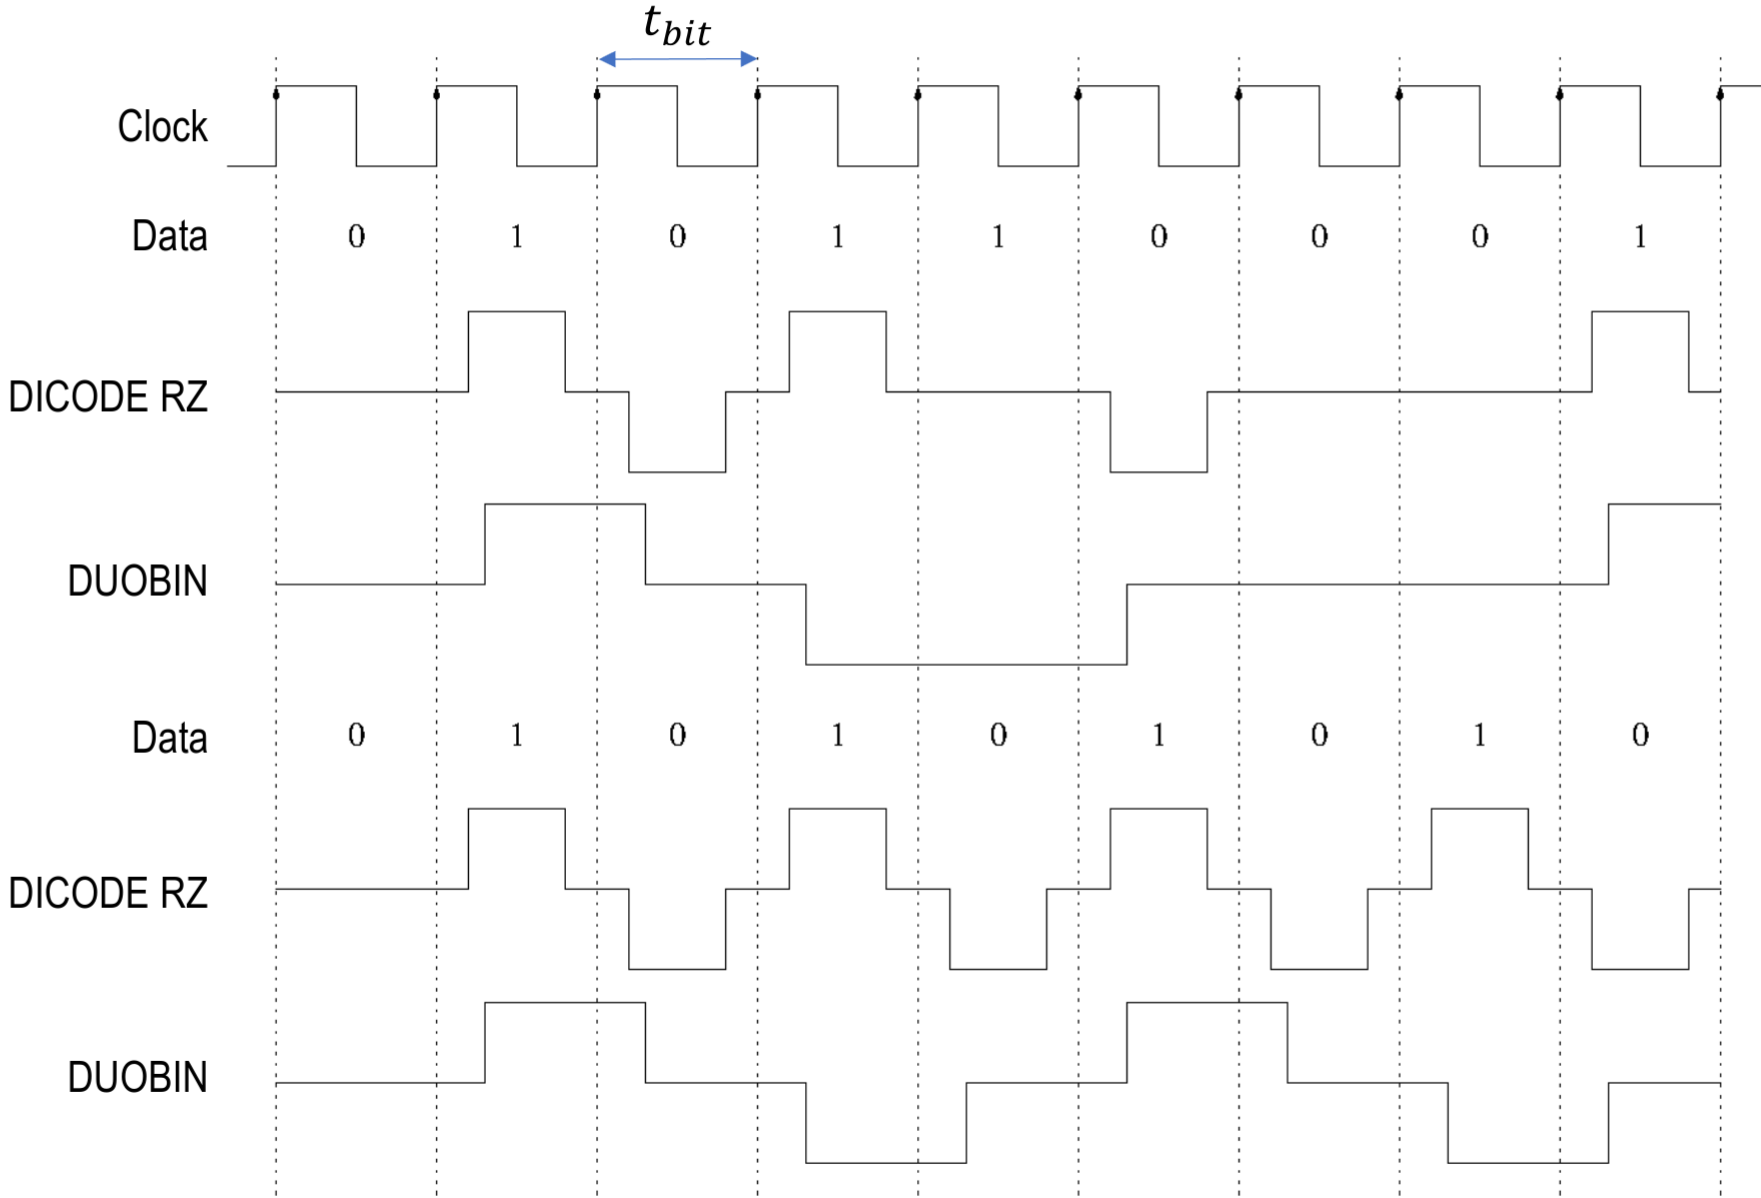
\includegraphics[scale=0.22]{../figures/dicode.png}
\end{center}

\subsubsection{MLT encoding}

This is significant because it used in Ethernet 100Base-TX (I would guess one of the thicknet standards).
For instance, MLT-3 has three logic levels:
\begin{itemize}
\item Logic 0: no change
\item Logic 1: output transition with alternate polarity
\end{itemize}

The bandiwdth is good as we get:
$$
f_\text{max} = \frac{f_\text{ck}}{4}
$$

\begin{center}
	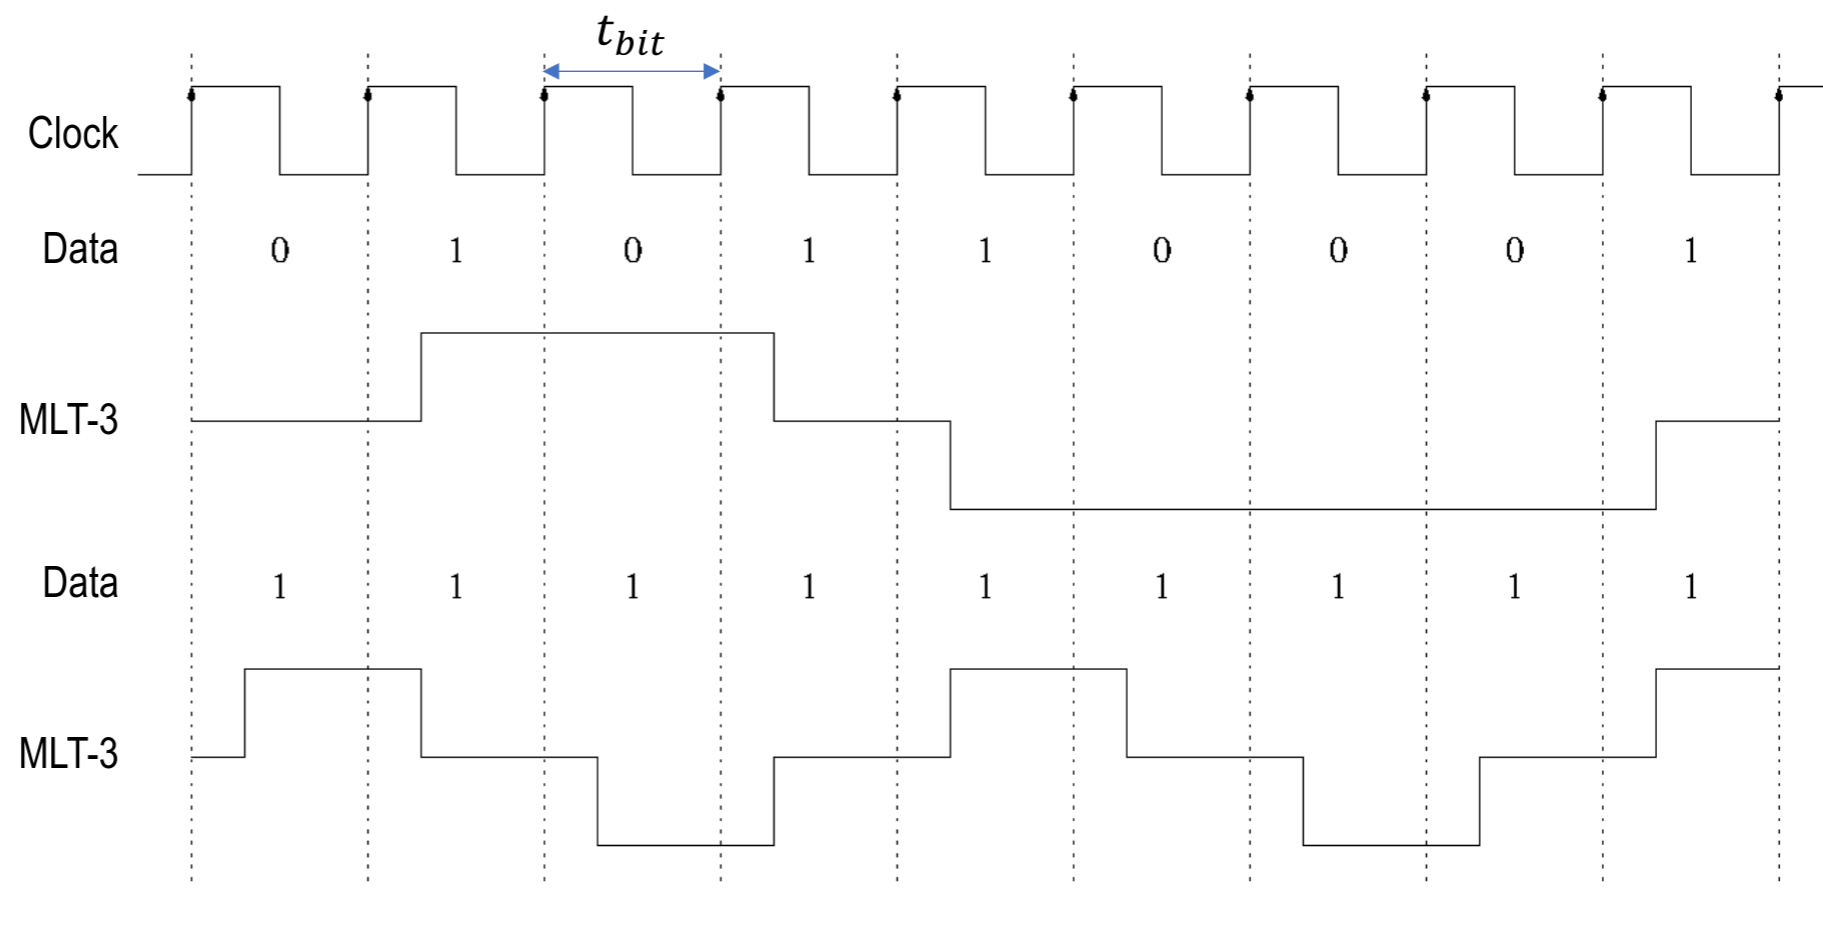
\includegraphics[scale=0.22]{../figures/mlt3.png}
\end{center}

\subsubsection{Manchester codes}

Also known as IEEE 802.3, \textbf{manchester codes} encode data via only transitions.
They can be obtained from NRZ-L (see 16.1.1) by XOR'ing with the clock.

\begin{itemize}
	\item Logic 1: low to high transition (L $\rightarrow$ H)
	\item Logic 0: high to low transition (H $\rightarrow$ L)
\end{itemize}

For the opposite encoding: 
\begin{itemize}
	\item Logic 1: high to low transition (H $\rightarrow$ L)
	\item Logic 0: low to high transition (L $\rightarrow$ H)
\end{itemize}

Transitions are guaranteed (which is good), but bandwidth of course suffers:
$$
f_\text{max} \leq f_\text{ck}
$$

\par\smallskip

There are some variations.

\begin{itemize}
	\item First off, \textbf{FM} (\textit{Frequency Modulation}). Also known as BiPhase or Differential Manchester Encoding:
		\begin{itemize}
			\item Logic 1: a transition at the beginning of the bit, followed by a transition in the middle of the bit
			\item Logic 0: a transition at the beginning of the bit
		\end{itemize}
	\item \textbf{MFM} is \textit{Modified Frequency Modulation}. The idea is to have different transition periods based on the value transmitted:
		\begin{itemize}
			\item Logic 1: a transition in the middle of the bit
			\item Logic 0: no transition if preceded by a 1, a transition at the beginning if preceded by a 0
		\end{itemize}
	\item Lastly we have \textbf{M2MF}, which is somehow named \textit{Modified Modified Frequency Modulation}. In particular, a clock pulse is only inserted between a pair of adjacent 0-bits if the first bit of the pair did not have a clock pulse inserted before it.

		This is wildly non standard as it seems the professor's slides interpret it differently (?). 
\end{itemize}

All of these guarantees transitions.

For bandiwdth, as we said, manchester is $f_\text{ck}$.
FM is also $f_\text{ck}$, whereas MFM and M2FM are:
$$
f_\text{max} = \frac{f_\text{ck}}{2}
$$

\begin{center}
	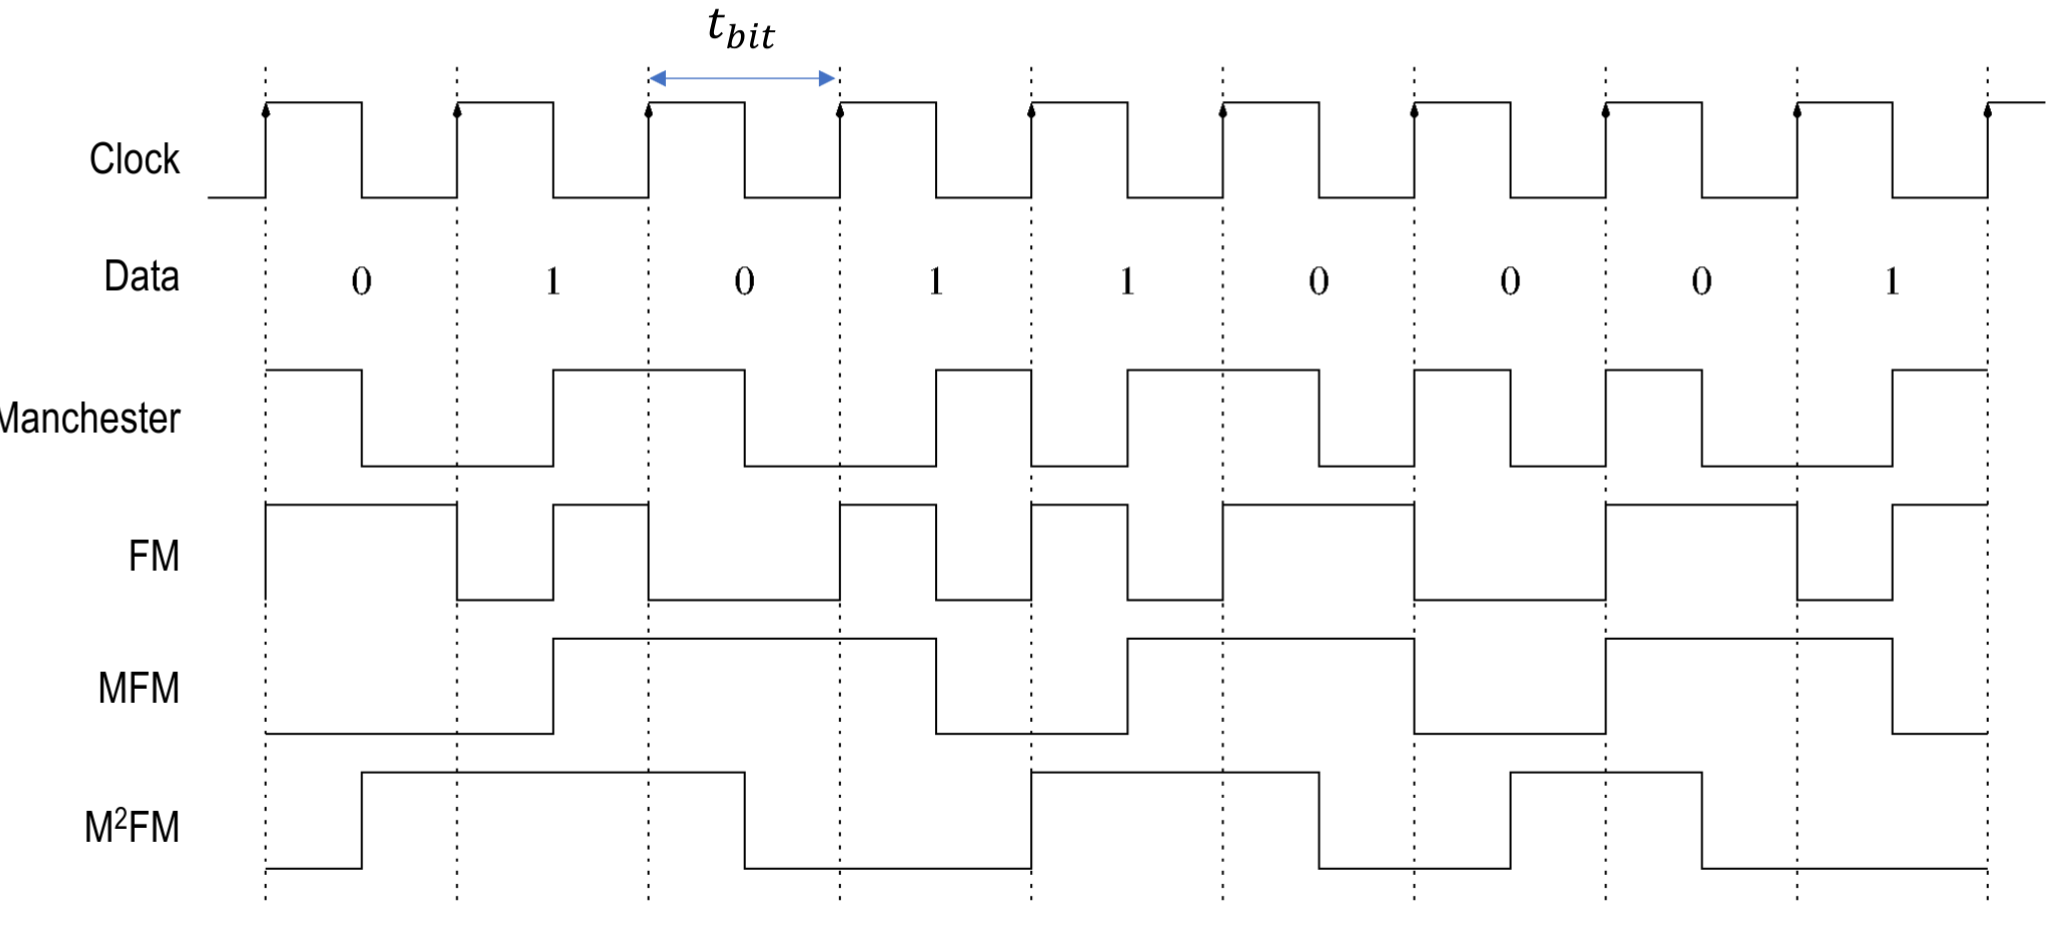
\includegraphics[scale=0.22]{../figures/manchester.png}
\end{center}

\subsubsection{Forcing transitions}

Some encodings show excellent characteristics, such as simplicity, low bandwidth, two voltage levels, but do not guarantee transitions.

We can solve this by forcing transitions into our data before encoding:
\begin{itemize}
	\item \textbf{xByB}: every $x$-bit block is replaced by a $y$-bit block, with $y > x$. Because of how the $y$ blocks are constructed this imposes the presence of transitions, is deterministic, but imposes a fixed overhead.

		Redundancy is used for transition insertions, but not at every bit: instead, they are guaranteed every $n$ bits. xByB can also be used for DC and low frequencies removal.

		\begin{center}
			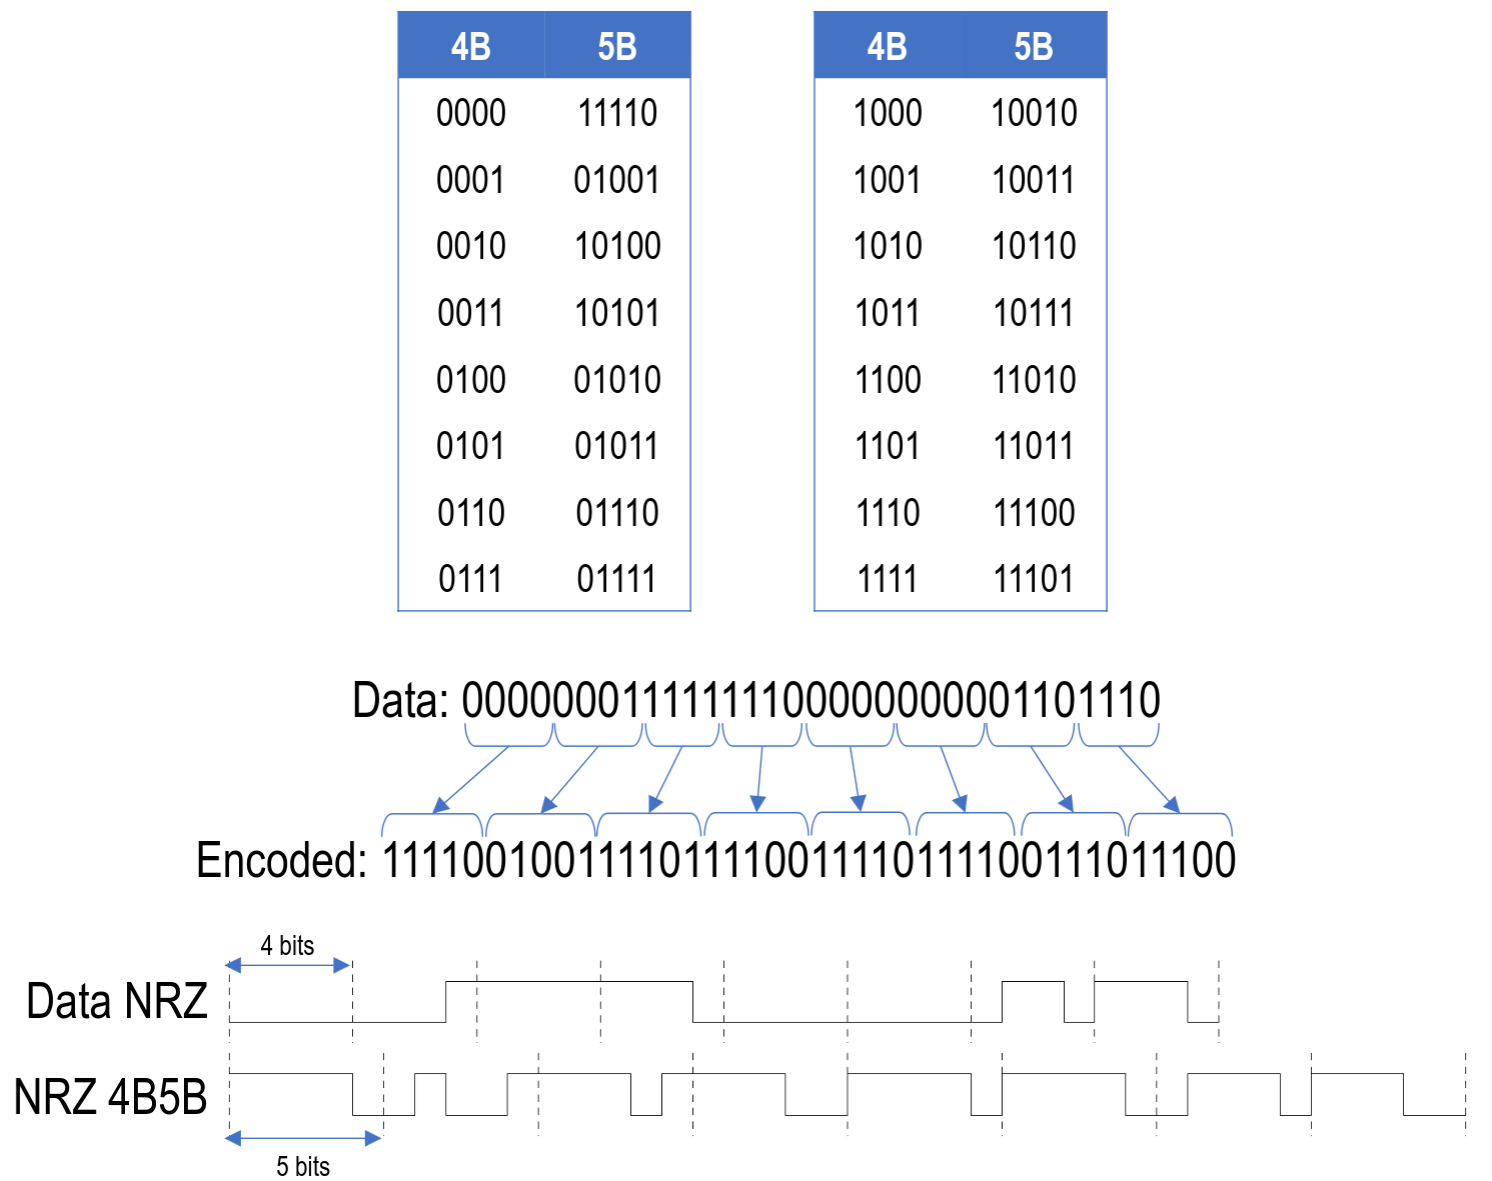
\includegraphics[scale=0.22]{../figures/xbyb.png}
		\end{center}

	There are a number of xByB codes, such as 3B4B, 4B5B, ecc... with different characteristics.
	They can all easily be implemented via LUTs.

\item \textbf{Bit stuffing} involves, every $n$ bits that don't cause a transition, to insert a bit that causes a transition.

	The value of $n$ is normally between 5 and 8, as the number of acceptable consecutive bits without a transition determined using the eye diagram.
	It differs depending on the protocol, with transmitter and receiver clocks re-synchronized at transitions.

	Of course at the receiver we have to notice if a bit that causes a transition is an actual data bit or a bit inserted via bit stuffing.
	This can be done simply by noticing the maximum number of hi (or low) bits was encountered, and the next bit as to be a 0 (or 1) of bitstuffing. If it isn't, it's likely an error or some kind of flag.

The main disadvantage of bit-stuffing is that the code rate is unpredictable; it depends on the data being transmitted.
\end{itemize}

\end{document}
